\documentclass [titlepage,a4paper]{article}

\usepackage[utf8]{inputenc}
\usepackage{makeidx}
\usepackage{graphicx}
\graphicspath{{figures/}}
\usepackage{amsmath}
\usepackage{theorem}
\usepackage[german]{babel}
\usepackage{cite}
\usepackage{textcomp}
\usepackage{fancyhdr}
\usepackage{float}
\usepackage{listings}
\usepackage{subcaption}

\usepackage{hyperref} 

\fancyhead{}
\fancyhead[LO]{\bfseries \rightmark}
\fancyfoot[LO]{\thepage}
\fancyfoot[CO]{}
\pagestyle{fancy}
\bibliographystyle{ieeetr}
\usepackage[title]{appendix}
\linespread{1.3}


\title{Ausstellung ''Link zur K.I."\\
Handbuch Interaktive Stationen\\
(WIP)}
\author{
    AG Reiterer\\
    Universität Konstanz
}

\date{Oktober 2019}

\makeindex



\begin{document}

\begin{titlepage}
\maketitle
\end{titlepage}


\pagenumbering{roman}

\tableofcontents

\pagebreak

\listoffigures 

\pagebreak

\pagenumbering{arabic}

\section{Allgemeines}

Alle Computer haben das Passwort \textit{link}.

\newpage
\section{Raum 1 ('Desktop')}

\subsection{Videoinstallation}

\subsubsection{Hardware}

\begin{itemize}
\item 3 Canon XEED WUX500ST Projektoren
\item 2 BenQ Projektoren
\item 1 Medienrechner
\item 1 Bildschirm
\end{itemize}

\subsubsection{Aufbau}

Die Canon-Beamer werden verwendet um die Projektionsflächen im Raum zu bespielen, die BenQ-Beamer für die Rückwand. Die Beamer sind gemeinsam mit einem Bildschirm zur Steuerung an dem Medienrechner angeschlossen, wober der Steuerungsbildschirm an die Grafikkarte angeschlossen werden muss.

(Abb. Video-Ins)

\subsubsection{Software}

Der Medienrechner steuert die Projektoren mit dem Programm Resolume an. Um die Wiedergabe zu starten muss in diesem ein Doppelklick auf dem Reiter über den Video-Vorschaubildern ausgeführt werden.

(Abb. Resolume)






\newpage
\section{Raum 2 ('Platine')}

\subsection{Überblick}

Für diesen Raum ist die Dokumentation nicht nach einzelnen Stationen gemäß ihrer Anordnung im Raum sortiert, sondern nach Art der Station, da viele nach dem gleichen Schema funktionieren. Die verschiedenen Stationen nach ihrer räumlichen Anordnung sind: 

\begin{figure} [H]
    \centering
    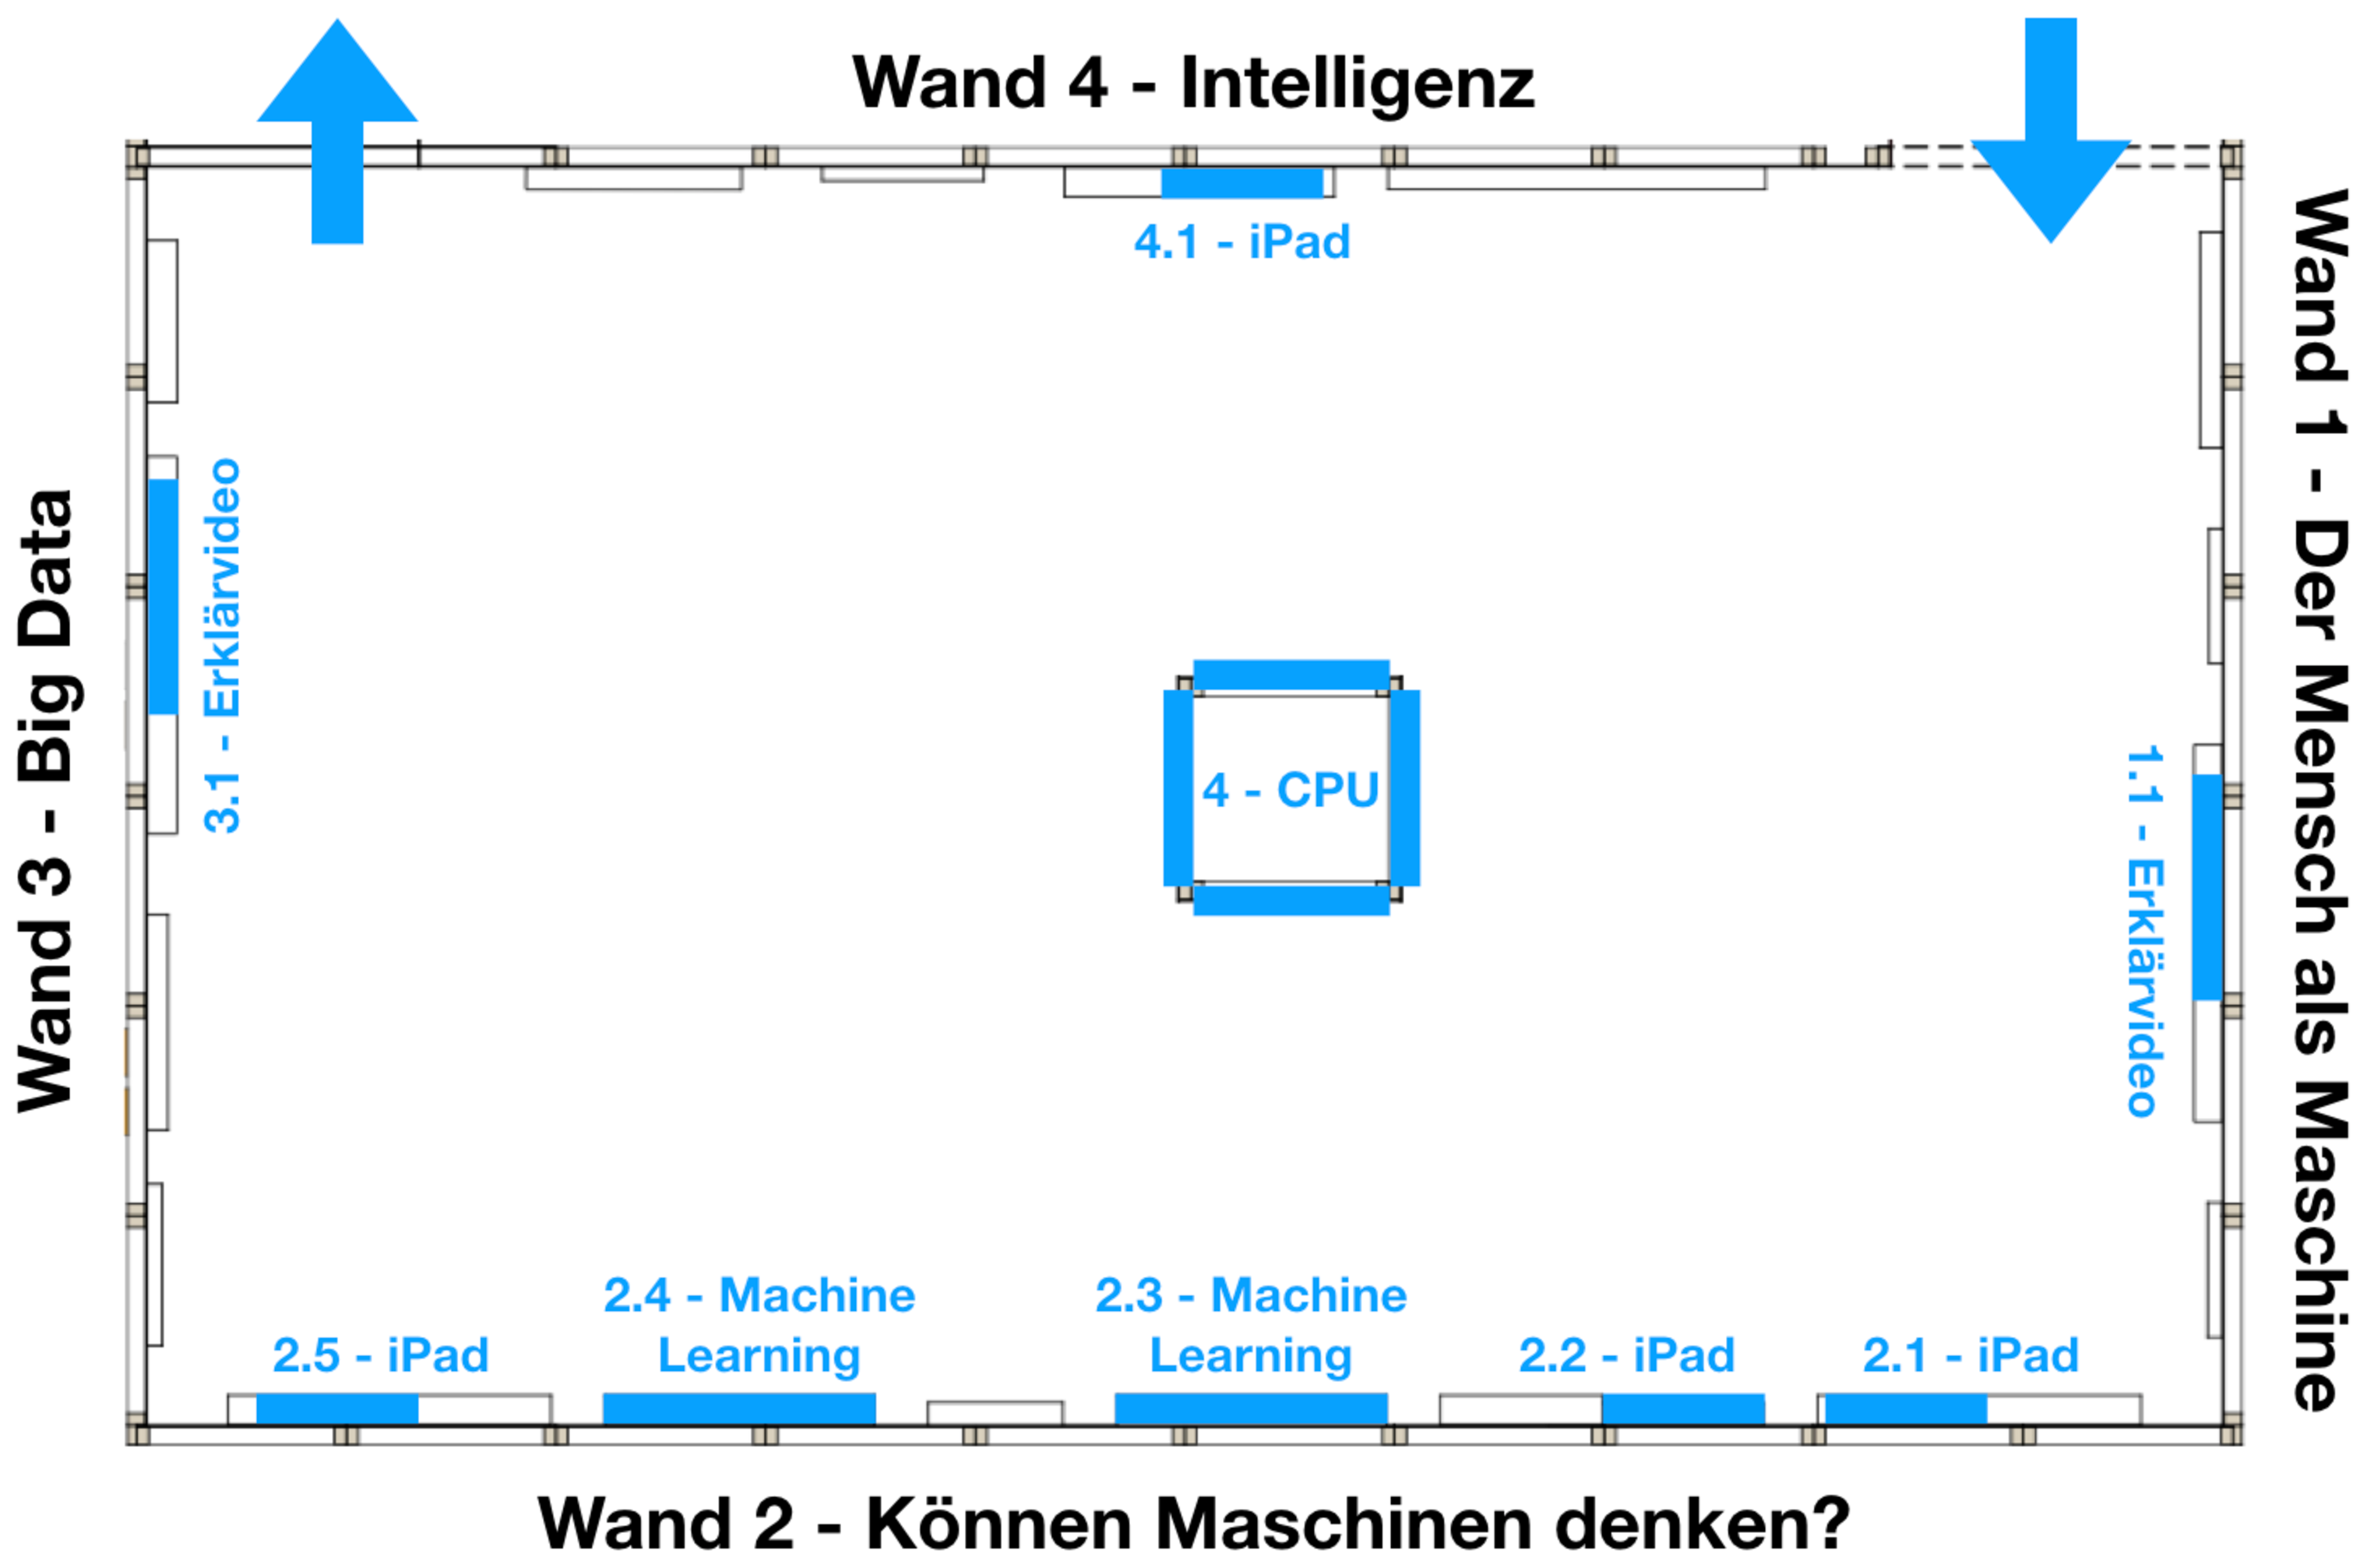
\includegraphics [width=1\textwidth]{images/Stationen_Platine.pdf}
    \caption{Räumliche Übersicht über die interaktiven Stationen in der Platine}
    \label{stationen_platine}
\end{figure}


\begin{itemize}
    \item Wand 1: Der Mensch als Maschine
        \begin{description}
            \item[1.1] Erklärvideo: Wandel des Menschenbildes
        \end{description}

    \item Wand 2: Können Maschinen denken?
        \begin{description}
            \item[2.1] iPad: Vertiefung zu Alan Turing
            \item[2.2] iPad: Chat mit ELIZA
            \item[2.3] Machine Learning - Neuronale Netzwerke
            \item[2.4] Machine Learning - Entscheidungsbaum
            \item[2.5] iPad: Die Dartmouth-Konferenz
        \end{description}

    \item Wand 3: AI - all inclusive?
        \begin{description}
            \item[3.1] Erklärvideo: Big Data 
        \end{description}

    \item Wand 4: Intelligenz
        \begin{description}
            \item[4.1] iPad: Intelligenztest
        \end{description}

    \item Raummitte: CPU
\end{itemize}

Im Folgenden sind nun die verschiedenen Arten Stationen jeweils erklärt. 

\subsection{Erklärvideos}

Die beiden Erklärvideos finden sich an Wand 1 und Wand 3. Die beiden Stationen bestehen jeweils aus einem Molitor Mediaplayer, der das Video, das auf einer SD-Karte gespeichert ist, abspielt. Über HDMI wird das Video auf den dazugehörigen 27-Zoll-Monitor übertragen. Über die vier bunten Kabel wird die dazugehörige Tonspur auf die Molitor Einhandhörer ausgegeben und umgekehrt das Signal, dass einer der Hörer abgenommen wurde, an den Mediaplayer weitergeleitet, sodass dieser das Video startet. \\
Auf der folgenden Website finden sich Kurzanleitungen für die Mediaplayer und Einhandhörer (unsere Einhandhörer sind von dem Modell USO; online verfügbar ist nur die Anleitung für einen Audioplayer, die lässt sich aber analog auf unsere Mediaplayer übertragen): \href{https://molitor-berlin.de/produkt-support/ }{https://molitor-berlin.de/produkt-support/}

\subsubsection{Hardware \& Verkabelung}

\begin{figure} [H]
    \centering
    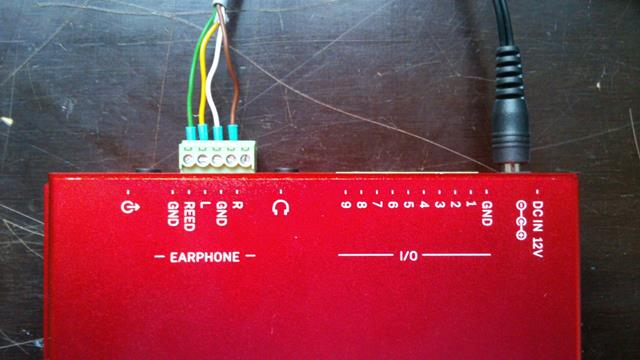
\includegraphics [width=1\textwidth]{images/AP01_Wiring_Detail.jpg}
    \caption{Verkabelung der Mediaplayer}
    \label{verkabelung_mediaplayer}
\end{figure}

$\rightarrow$ Skizze mit Anschlüssen/ Verbindungen

Mediaplayer:
\begin{itemize}
    \item Stromanschluss
    \item HDMI-Anschluss $\rightarrow$ Monitor
    \item Audioausgang (Phönixstecker) $\rightarrow$ Einhandhörer (jeweils alle 4 Farben; zwei Kabel je Farbe in einen Eingang)
    \item SD-Karte
\end{itemize}



Monitor:
- Strom
- HDMI $\leftarrow$ Mediaplayer

Einhandhörer:
- Audioeingang (bunte Kabel) $\leftarrow$ Mediaplayer

\subsubsection{Software \& Einstellungen}

Die SD-Karte wird über einen Windows-Rechner mit den entsprechenden Videos bespielt. Auch der idle-Screen wird hier als Video abgespeichert.

\subsection{iPads}

\subsubsection{Hardware \& Verkabelung}

Die iPads werden einfach dauerhaft über ihre Ladekabel an den Strom angeschlossen. Eine Besonderheit gibt es bei Station 2.2 (Eliza): Hier wird an das iPad der Adapter angeschlossen, und an den dann einmal die Tastatur und das Ladekabel. Die Tastatur funtkioniert nur, wenn das Ladekabel auch wirklich mit dem Strom verbunden ist.

\subsubsection{Software \& Einstellungen}

Auf den iPads öffnet man die App "safully", die als Fullscreen-Webbrowser funktioniert. In dieser gibt man dann die Url für die jeweilige Station ein. Die Ports, auf die die Urls enden, sind: \begin{description}
    \item[8001] iPad 4.1 - IQ-Test 
    \item[8003] iPad 2.1 - Vertiefung Alan Turing
    \item[8004] iPad 2.5 - Vertiefung Dartmouth Konferenz
    \item[8007] iPad 2.2 - Eliza 
\end{description}

Per 3-fach-Klick auf den Home-Button wird anschließend der geführte Modus aktiviert, der verhindert, dass die Besucher andere Apps öffnen können. 

\subsection{Machine Learning Stationen}

\subsubsection{Hardware \& Verkabelung}

USB A (-> Rechner/ NUC) auf B (-> Touchscreen)
Touchscreen - HDMI - Rechner/ NUC
Touchscreen - Strom
Rechner/ NUC - Strom

\subsubsection{Software \& Einstellungen}

TOBI?

Die Machine-Learning-Stationen werden lokal gehostet. Dazu müssen auf den jeweiligen Rechnern Skripte ausgeführt werden:

\begin{itemize}
\item Auf der Station für Neuronale Netzwerke muss mit der Tastenkombination 'Windows + T' ein Terminal geöffnet werden. In diesem muss der Befehl \begin{verbatim}
./strtNN
\end{verbatim} ausgeführt werden.
\item Auf der Station für Entscheidungsbäume muss die Datei (Insert name here?) auf dem Desktop mit einem Rechtsklick $\rightarrow$ 'In Windows Powershell ausführen' geöffnet werden. Danach wird Chrome mit der Verknüpfung auf dem Desktop geöffnet, um den Inhalt anzuzeigen.
\end{itemize}

Die Ports, auf die die Urls enden, sind: \begin{description}
    \item[8005] Machine Learning 2.4 - Entscheidungsbaum
    \item[8006] Machine Learning 2.3 - Neuronales Netzwerk
\end{description}

\subsection{CPU}

\subsubsection{Hardware \& Verkabelung}

Rechner $\rightarrow$ Strom
        $\rightarrow$ 4x Monitoranschluss (1x HDMI + 3x Displayport + Adapter (?))

\subsubsection{Software \& Einstellungen}

\paragraph{Server für iPads}
TOBI?

\paragraph{Betreiben der CPU-Bildschirme mit Resolume}
TOBI?


\newpage
\section{Raum 3 ('Server')}

\subsection{Medizinquiz}

\subsubsection{Hardware \& Verkabelung}

\subsubsection{Software \& Einstellungen}

Die Ports, auf die die Urls enden, sind: \begin{description}
    \item[8008] Medizinquiz
\end{description}

\newpage
\section{Raum 4 ('Cloud')}

\subsection{Chatbot 'Aski'}

\subsubsection{Hardware}

\begin{itemize}
\item 5 Surface Pro 6
\item 5 4k-Fernseher
\item USB-Schlösser
\end{itemize}

\subsubsection{Aufbau}

Die Fernseher und Tablets werden in den Seilen als Paare montiert und per Videokabel (Mini-Display Port auf HDMI, 4k-fähig) verbunden. Die USB-Slots werden mit dem beiliegenden Schloss-System vor ungewünschten Zugriffen geschützt.

\subsubsection{Software}

Die Surfaces stellen ihren Inhalt selbst über einen npm-Server bereit. Dieser kann auf dem Desktop mit einem Rechtsklick $\rightarrow$ 'Mit Windows Powershell ausführen' auf die Datei 'Starte Aski' gestartet werden. Der Inhalt kann dann mit Chrome angezeigt werden, wobei Chrome über die Verknüpfung auf dem Desktop gestartet werden sollte. Dabei muss eine Maus an das Surface angeschlossen sein, um das Anzeigefenster für Chat und Video auf den Fernseher zu bewegen.

\end{document}
